\documentclass{sigchi-ext}
% Please be sure that you have the dependencies (i.e., additional
% LaTeX packages) to compile this example.
\usepackage[T1]{fontenc}
\usepackage{textcomp}
\usepackage[scaled=.92]{helvet} % for proper fonts
\usepackage{graphicx} % for EPS use the graphics package instead
\usepackage{balance}  % for useful for balancing the last columns
\usepackage{booktabs} % for pretty table rules
\usepackage{ccicons}  % for Creative Commons citation icons
\usepackage{ragged2e} % for tighter hyphenation

% Some optional stuff you might like/need.
% \usepackage{marginnote} 
% \usepackage[shortlabels]{enumitem}
% \usepackage{paralist}
% \usepackage[utf8]{inputenc} % for a UTF8 editor only

%% EXAMPLE BEGIN -- HOW TO OVERRIDE THE DEFAULT COPYRIGHT STRIP --
% \copyrightinfo{Permission to make digital or hard copies of all or
% part of this work for personal or classroom use is granted without
% fee provided that copies are not made or distributed for profit or
% commercial advantage and that copies bear this notice and the full
% citation on the first page. Copyrights for components of this work
% owned by others than ACM must be honored. Abstracting with credit is
% permitted. To copy otherwise, or republish, to post on servers or to
% redistribute to lists, requires prior specific permission and/or a
% fee. Request permissions from permissions@acm.org.\\
% {\emph{CHI'14}}, April 26--May 1, 2014, Toronto, Canada. \\
% Copyright \copyright~2014 ACM ISBN/14/04...\$15.00. \\
% DOI string from ACM form confirmation}
%% EXAMPLE END

% Paper metadata (use plain text, for PDF inclusion and later
% re-using, if desired).  Use \emtpyauthor when submitting for review
% so you remain anonymous.
\def\plaintitle{Shared Story: Constructing Identity and Local Community through Tangible Exploration} \def\plainauthor{Diego Salvatierra, Po Tsui}
\def\emptyauthor{}
\def\plainkeywords{Identity construction environment; child-computer interaction; youth; education; tangible user interfaces}
\def\plaingeneralterms{Documentation, Standardization}

\title{Shared Story: Constructing Identity and Local Community through Tangible Exploration}

\numberofauthors{2}
% Notice how author names are alternately typesetted to appear ordered
% in 2-column format; i.e., the first 4 autors on the first column and
% the other 4 auhors on the second column. Actually, it's up to you to
% strictly adhere to this author notation.
\author{%
  \alignauthor{%
    \textbf{Diego Salvatierra}\\
    \affaddr{Stanford University} \\
    \affaddr{Stanford, CA 94305, USA} \\
    \email{dsalva@stanford.edu} }\alignauthor{%
    \textbf{Po Tsui}\\
    \affaddr{Stanford University}\\
    \affaddr{Stanford, CA 94305, USA}\\
    \email{potsui@stanford.edu} } }

% Make sure hyperref comes last of your loaded packages, to give it a
% fighting chance of not being over-written, since its job is to
% redefine many LaTeX commands.
\definecolor{linkColor}{RGB}{6,125,233}
\hypersetup{%
  pdftitle={\plaintitle},
%  pdfauthor={\plainauthor},
  pdfauthor={\emptyauthor},
  pdfkeywords={\plainkeywords},
  bookmarksnumbered,
  pdfstartview={FitH},
  colorlinks,
  citecolor=black,
  filecolor=black,
  linkcolor=black,
  urlcolor=linkColor,
  breaklinks=true,
}

% \reversemarginpar%

\begin{document}

%% For the camera ready, use the commands provided by the ACM in the Permission Release Form.
%\CopyrightYear{2007}
%\setcopyright{rightsretained}
%\conferenceinfo{WOODSTOCK}{'97 El Paso, Texas USA}
%\isbn{0-12345-67-8/90/01}
%\doi{http://dx.doi.org/10.1145/2858036.2858119}
%% Then override the default copyright message with the \acmcopyright command.
%\copyrightinfo{\acmcopyright}

\maketitle

% Uncomment to disable hyphenation (not recommended)
% https://twitter.com/anjirokhan/status/546046683331973120
\RaggedRight{} 

% Do not change the page size or page settings.
\begin{abstract}
Shared Story aims to help middle and high school students reflect on their life stories and share these stories with others in their community. Students in highly segregated communities rarely have a chance to share their life stories with people from other backgrounds. They may also be unaware of how their life story has been shaped by their community history. Shared Story is a collaborative map on a tangible user interface (TUI) table that allows individuals to construct important events in their lives and their communities, which would then be saved onto a collaborative map online. By viewing the events placed by others, young learners will become aware of how others in their community lead their lives and what places and events have shaped them.
\end{abstract}

\keywords{\plainkeywords}

\category{H.5.m}{Information interfaces and presentation (e.g.,
  HCI)}{Miscellaneous}\category{See}{\url{http://acm.org/about/class/1998/}}{for
  full list of ACM classifiers. This section is required.}

\section{Introduction}
In today's classrooms, too little time is spent on reflection and personal history. There also exist limited means of sharing and engaging with personal history, and a general lack of knowledge of community history, which in turns exacerbates the division caused by urban segregation. We are motivated to address these issues by proposing a design that would enable learners, primarily of adolescent age, to construct and share their life stories and explore how their community's history connects with these stories.

Our learning goals are as follows:
\begin{enumerate}\compresslist
	\item \textbf{Engage in personal reflection which acknowledges their own historicity and dynamic self}: Learners will reflect and construct their own personal stories.
	\item \textbf{Engage in local community and its history}: Learners will collaboratively discover and contribute important events and places within their local community, and how these things intersect with their own story.
	\item \textbf{Develop peer empathy}: Learners will explore the life stories of peers in their own or nearby communities and develop a deeper understanding of the lives of others outside their own selves.
\end{enumerate}

\begin{marginfigure}[-25pc]
  \begin{minipage}{\marginparwidth}
    \centering
    \includegraphics[width=0.9\marginparwidth]{figures/map}
    \caption{School segregation in the Bay Area. Source: Vox, \textit{We can draw school zones to make classrooms less segregated. This is how well your district does.} 2018.}~\label{fig:bay-area-map}
  \end{minipage}
\end{marginfigure}

\section{Theoretical Framework}
Our project is primarily rooted in critical pedagogy. Paulo Freire (2006) argues that learners should become aware of their world and its social and political conditions - through what he calls "a constant unveiling of reality" - and their position within it. The reality we help learners unveil is that of their surrounding community and their own personal histories. Freire stresses that students should not simply explore, but rather construct their world, through what he terms "praxis." He recognizes that "reality is a process"; as such, students must come to understand that they are simultaneously part of this dynamic reality and can change it. This is the process of \textit{conscientiza\c{c}\~{a}o}. By allowing learners to construct personally significant places and events on a physical timeline and map, we help students undertake this process of creating their reality.

We also draw on the psychological theories of Erik Erikson (1962) for understanding how our target learners, middle- and high-school students, view themselves. Erikson describes the psychosocial crises that individuals experience in different stages of life. During the identity vs. role confusion stage experienced by adolescents, they feel "a sense of the irreversibility of significant events and an often urgent need to understand fully and quickly what kind of happenings in reality and in thought determine others, and why." Adolescents seek historical frameworks, identities, and roles in which to make sense of who they are. Through our project, we aim to help them understand the events that, to quote Erikson, "determine others" and themselves.

Lastly, we build on the concept of restructurations as put forward by Wilensky and Papert (2010), which are new symbols and structures of knowledge that make it possible for learners to achieve previously difficult tasks. Sharing one's life history most commonly exists today as written and oral narratives. Our project, instead, allows students to easily share the story of their life and their community, especially for those without considerable writing or artistic skills in other contexts. As it aggregates data, this approach also allows for macro-level patterns and insights to emerge, which abides by Wilensky's power principle.

The United States, like many other countries, suffers from high segregation in schools by race and class. As shown in Fig. 1, the Bay Area is not immune from these dynamics. As our project help students become aware of the lived experiences of others in nearby communities, it is worth referring to studies that demonstrate how one can bridge social divides among different school communities. Lopez and Nastasi (2012) share their experience with a project that brought together youth from suburban and urban school districts. Students from different districts shared conversations on their own identities, followed by a collaborative project on how to improve their community. The authors found that "when curriculum and pedagogy help students to understand their own identities, the identities of their peers, and methods for collaboration, students are prepared for democratic participation." Although our project does not yet replicate the aforementioned methods of collaboration, we facilitate the first two pedagogical components put forward by these authors: helping students understand their own identities and those of their peers. 

\section{Technological Framework}
Learners engage with our learning goals through what Papert (1980) calls an "object-to-think-with," which help learners grasp certain abstract concepts through tangible means and share ideas with the world. Our project builds on his constructionist framework by allowing learners to create physical representations of their memories and perceptions of their surroundings. 

Drawing on Horn's work (2013), particularly his study of table top exhibits in museums, our use of a TUI table evokes cultural forms around socialization and play through a more familiar and child- (rather than parent-) driven design. The "associated resources of video game play" that exist in table top play invite both individual and group engagement. Additionally, the work of Petrelli, Whittaker, and Brockmeier (2008) on mementos and autotopographies indicate that physical mementos play a large role in triggering memories, and suggest potential in augmenting objects with digital memories. In our design, physical 3D-printed representations of events and places are augmented with digital (textual and symbolic) representations. In such a way we allow for "meaning construction" through tangible interaction.

Finally, we introduce a shared screen with aggregated stories overlaid together on a single map as a way to create a multi-user environment which encourages community building and lends the user a social context in which to construct their personal history. The collaborative maps become an object for students to reflect upon their lives and their communities, and to share them publicly with the world.

\section{Related Work: Identity Construction Environments}

Marina Umaschi Bers (2009) has conducted extensive work on what she terms "Identity Construction Environments" (ICE), which are "technological tools purposefully designed to afford opportunities for exploring identity and engaging in reflection and discussion about personal and moral values." We abide by the five principles she puts forth, which involve purposeful design to help young people learn about and construct their identity through community, storytelling, and dynamic objects representing the self:

\begin{enumerate}\compresslist
	\item They are purposefully designed to help young people learn about their identity, particularly personal and moral values.
	\item They are designed on a theoretical model that positions identity as a complex and dynamic construction composed by conflicting values.
	\item They afford opportunities for learners to design dynamic computational objects and spaces representing aspects of the self.	 							
	\item They offer opportunities for storytelling and they elicit narratives about the self.
	\item They support the creation of and participation in a community. No sense of self develops in a social vacuum.
\end{enumerate}

We study Zora, a multi-user virtual environment that allows learners to design and participate within a graphical virtual city and its social organization, and the pivotal work behind Bers's ideas within this field. In this virtual environment, individuals create avatars of themselves, design their own living spaces, engage collaboratively in the construction and maintenance of their microcommunity. Zora also contains a "collaborative values dictionary" through which individuals can explore their personal and moral values. 

Our project parallels some of the same elements found in Zora. Through our design, learners reflect on abstract histories, perceptions of their communities, and personal values in concrete ways through objects-to-think-with. The selection of what to display and share physically is an active process of self-reflection and construction of what is important to that individual. We make use of narrative therapy, which casts storytelling as the means through which construct ourselves and our identities.

However, Zora is situated within a virtual world and thus one level removed from the physical community in which the student lives and has developed personal history. We in contrast use the actual neighborhood as touchpoints for reflection and transforming action. We ground our users to their immediate surroundings and aim in Freirean fashion to lead to direct action upon the learner's world. By actively constructing and sharing their neighborhoods, students learn about the actual history of their immediate surrounding community and the lives of their peers. In doing so, we also differ from Zora's approach by placing an emphasis on the historicity of the individual and the community. We aim for learners to make sense of their own lived experiences and recognize themselves in the context of their community and family history, as standing on the backs of their ancestors. The design allows for users to view their construction as one whole, through which macro-level insights can emerge. Finally, our tangible user interface embodies a harder constructionist approach, wherein the abstract are represented by physical objects to be touched and manipulated by the hand. The physical placement of three-dimensional markers on our TUI map represents not only the physical construction of an individual's identity, but also a sociopolitical assertion of physical existence in the real world. 

\section{Design}
Our project is a collection of collaborative maps and timeline on a tangible user interface (TUI). Its features allow learners the following actions.

\subsection{Choosing your map}

The maps themselves portray different communities that students may belong to. In the current prototype we include three maps: Stanford University, Palo Alto, and East Palo Alto. The maps are stylized watercolor versions of regular  Google Maps, making them friendlier and more attractive. The maps include the location of major landmarks, recreational areas, and streets, as well as large schools in the area, to make it easier for students to locate the places that are important in their lives. 

The maps are displayed on a screen at the top of a wooden table. On this table, learners may place several different physical pieces. Students can choose the map most relevant to them by placing one of three wooden map pieces (one for each map) on the top left-hand corner of the map, on a special square indicated for that purpose. Institutions hosting a Shared Story table could add important local historical events, thus making students more aware of how their community's history intersects with their own lives. 

\subsection{Placing events on map}

These different event pieces correspond to different categories of events and places that may be significant to students. When a physical event piece  is placed on the table, a digital icon appears near it on the map. Learners can move the physical icon to maneuver the digital icon on screen. Each physical icon (left) corresponds to the following digital icon, and the following categories of events.

\subsection{Adding event descriptions}

Once an event icon has been placed on the map, learners can type a small description next to it using a keyboard connected to the table. In the future, we hope to enable learners to upload photos and artwork as an additional complement to the icons. 

\subsection{Adding events to timeline}

Besides the map itself, we have also embedded an unlabeled timeline on the screen. This allows students who want to save events on a timescale to do so - they can add an event to the timeline, and type in the time that it happened.

\subsection{Saving and sharing the map}

After a user is satisfied with all the events she has added to the map, she can save the map by placing a wooden icon labeled "save" on the map. This immediately freezes the map and uploads it to an online database. From the online database, a shared map can be generated that shows all of the events previous users have inputted, as shown below. This shared map is available online (Fig. 2) and can be projected or shown onto a separate screen. Since the table will be located in a public shared space, such as a museum or a public library, learners will be able to see the events put on the shared map by other users.

\begin{marginfigure}[-57pc]
  \begin{minipage}{\marginparwidth}
    \centering
    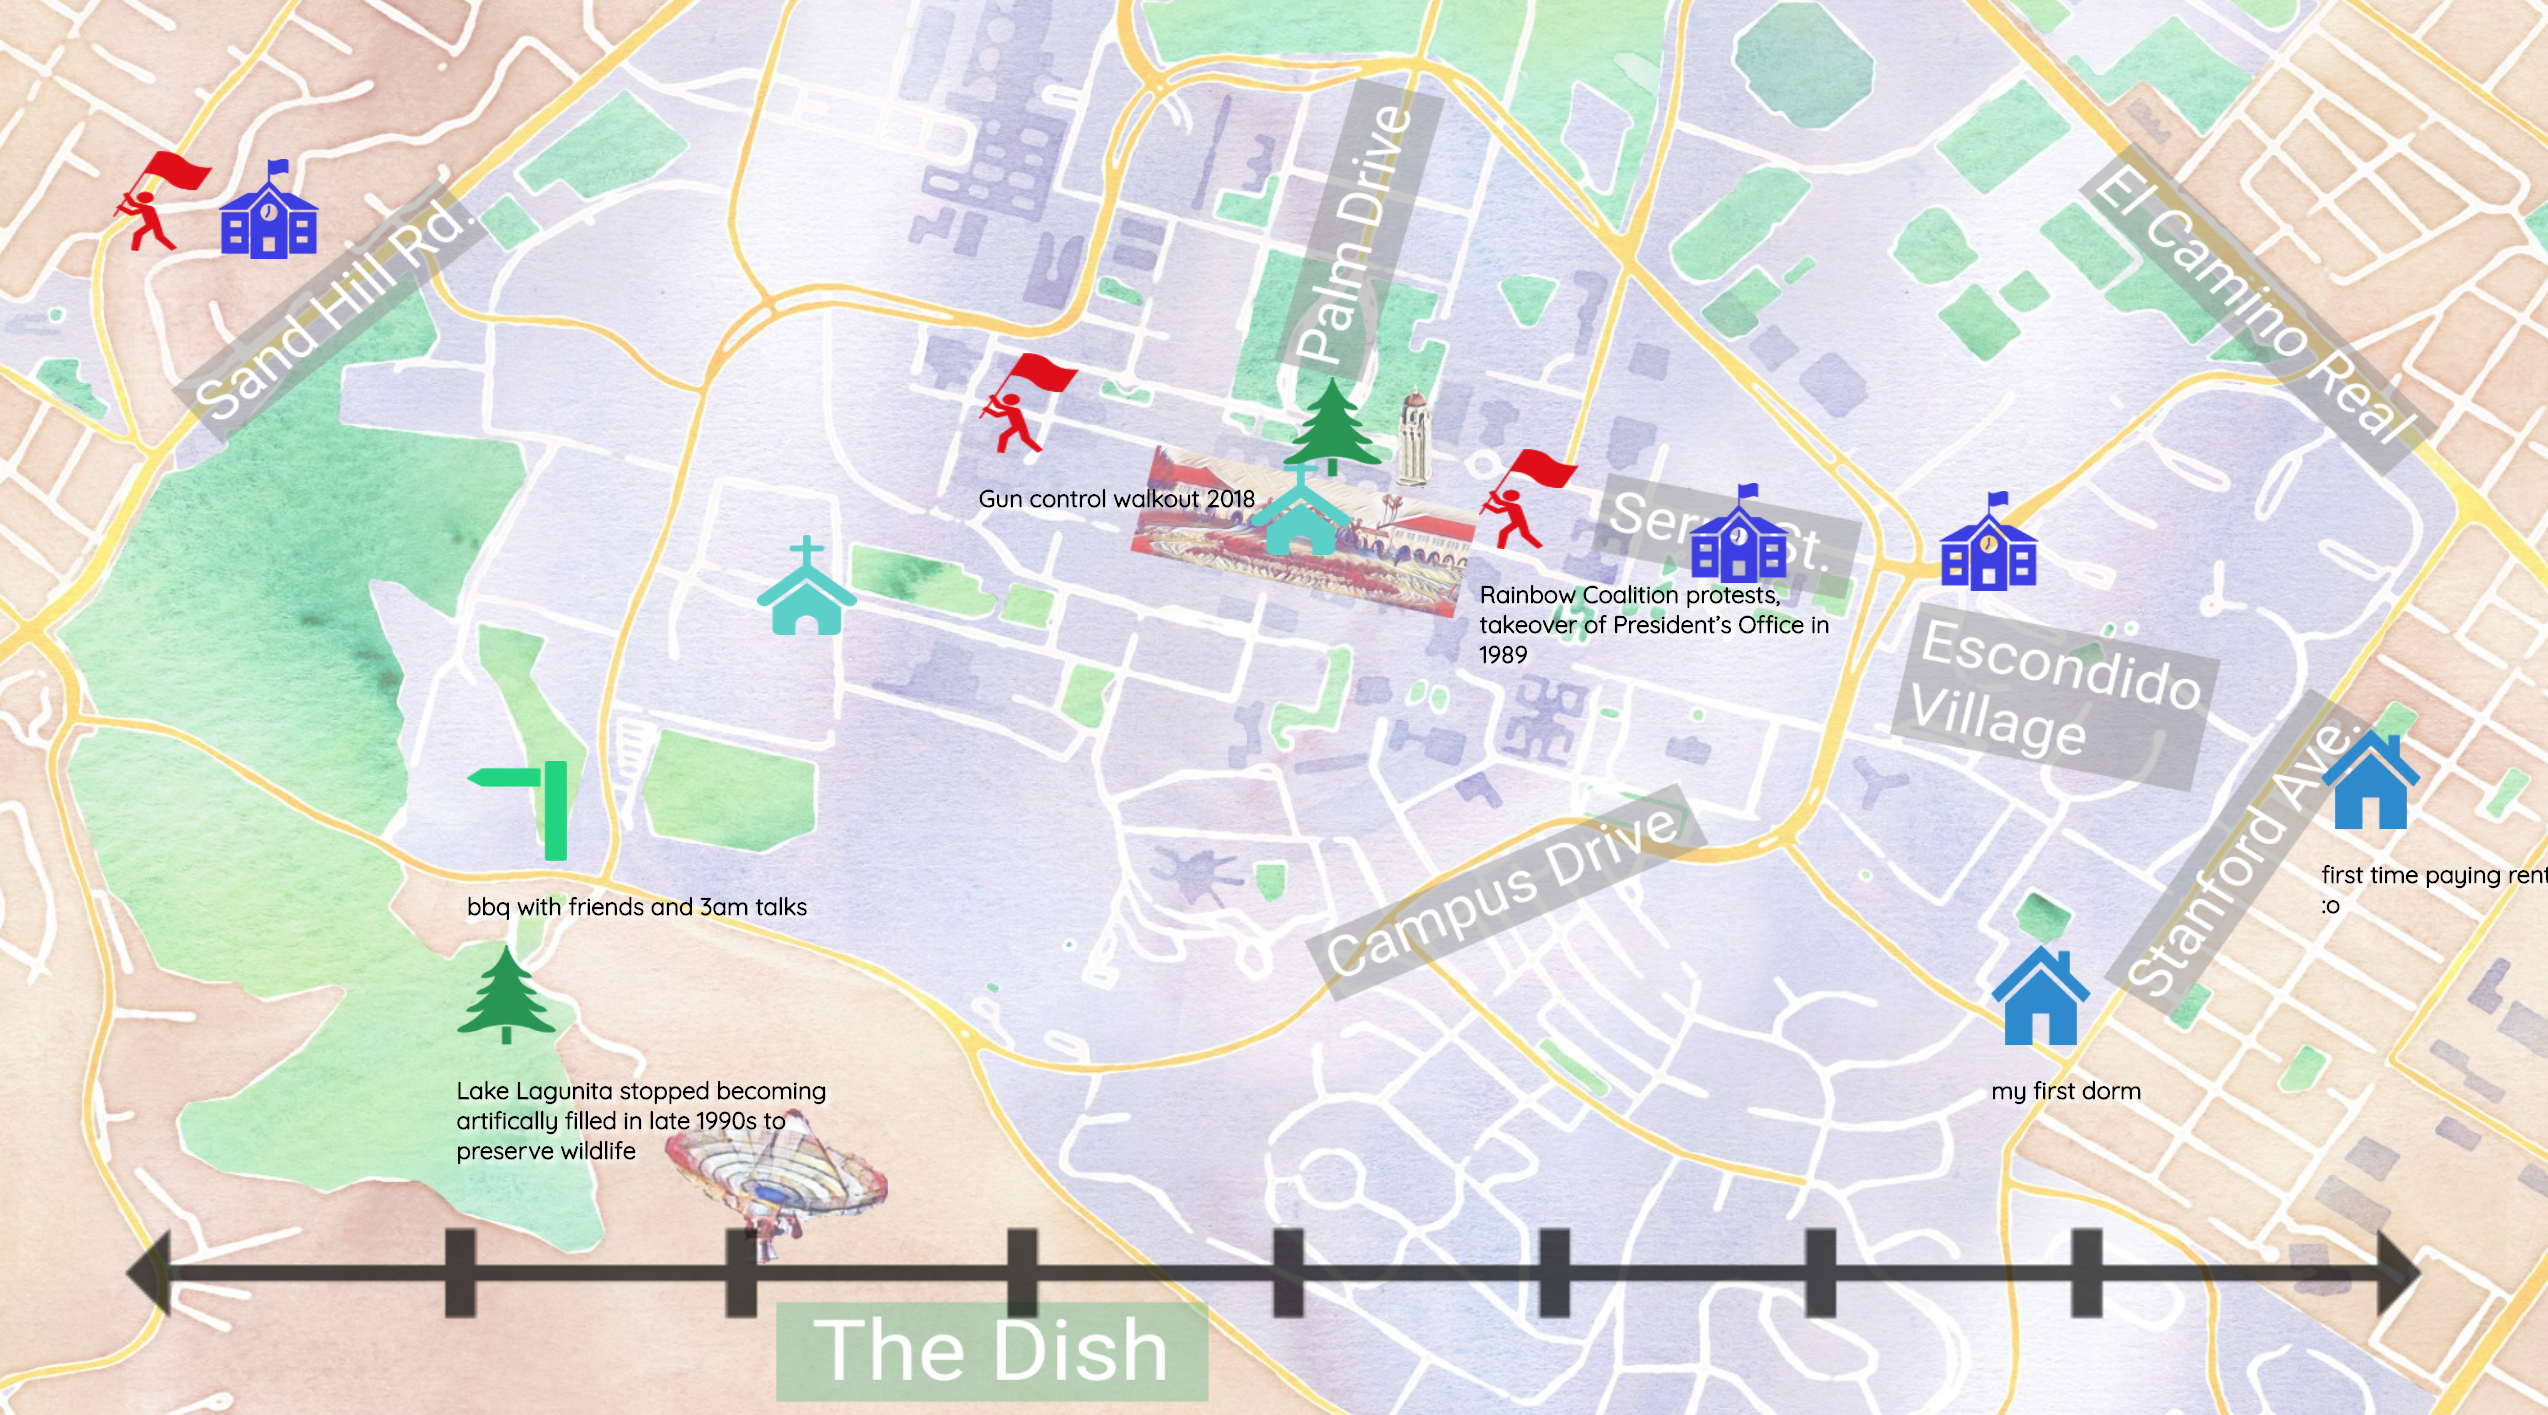
\includegraphics[width=0.9\marginparwidth]{figures/web}
    \caption{Web view: aggragated stories on a shared map}~\label{fig:web}
  \end{minipage}
\end{marginfigure}

\begin{marginfigure}[-36pc]
  \begin{minipage}{\marginparwidth}
    \centering
    \includegraphics[width=0.9\marginparwidth]{figures/tui}
    \caption{Our tangible user interface table design}~\label{fig:tui}
  \end{minipage}
\end{marginfigure}

\begin{marginfigure}[-14pc]
  \begin{minipage}{\marginparwidth}
    \centering
    \includegraphics[width=0.9\marginparwidth]{figures/table}
    \caption{The Shared Story table and web view}~\label{fig:table}
  \end{minipage}
\end{marginfigure}

\section{Technical Construction}

Our tangible user interface table is inspired by the design put forth by Konrad and Jung (2012). In this tangible user interface, objects are placed on the semi-transparent surface. These pieces have fiducials (visual patterns generated by the Reactivision software) pasted in the bottom. These are read by a camera at the bottom of the table. To make readability easier given the ambient light that seeps through the semi-transparent screen, the camera has an infrared filter, and infrared lights are shone onto the bottom of the screen. At the same time, a projector placed at the bottom of the table projects the desired screen onto the semi-transparent surface. 

The major difference in our design (Fig. 3 and 4) is that the camera we use is connected to a laptop outside the table box, as well as a keyboard for learners to input their event description. In the Shared Story exhibit the laptop would be hidden from view, with only the keyboard accessible. We also built a wood-paneled box for the table, which increases the darkness inside the TUI and makes fiducial recognition easier. Lastly, similarly to other tables built  at the Transformative Learning Technologies Lab (TLTL) at Stanford, we put two panels of 20 infrared lights each, one on each internal side of the table, that each project onto one half of the screen. This also makes fiducial recognition easier, as the amount of infrared light is focused and controlled.

We use the ReactiVision library to recognize these fiducial patterns, which are then streamed as input to our Processing application that runs the graphics on the TUI table. Whenever a user saves their constructed map, the data is sent from the Processing application to our Firebase database. The aggregated data is viewable at \url{sharedstory.herokuapp.com}, a Node.js server we built and hosted on Heroku.

\section{Conclusion}
We propose Shared Story as a social tangible interface design project that allows middle and high school students to reflect on and share their life stories with others in their community. We build on constructionist principles, emphasize Freire's focus on conscientization and Erikson's theories of identity formation, and learn from prior work in identity construction environments. Our goal is to restructure the narrative form such that learners can more easily and powerfully engage in the active construction of their personal histories and reflection on their dynamic identities, while situated within the social context of their local community. Users place physical objects representing important places and events in their lives and manipulate them through tangible and digital means, moving them around the map projected onto our table and adding text via a connected keyboard. They can then save their constructions and share them publicly; the collection of student contributions within a given local community can then be explored.

\section{Acknowledgements}
We thank Paulo Blikstein, Richard Davis, Chris Proctor, Veronica Lin, and the rest of the Beyond Bits and Atoms teaching team for their continuous support.

%\balance{} 

\section{References}
\vspace{4mm}

\begin{enumerate}\compresslist
	\item Bers, Marina Umaschi. (2001) Identity Construction Environments: Developing Personal and Moral Values Through the Design of a Virtual City, The Journal of the Learning Sciences, 10:4, 365-415.

	\item Bers, M. U. and Chau, C. (2006). Fostering Civic Engagement by Building a Virtual City. Journal of Computer-Mediated Communication, 11: 748–770.

	\item Erikson, E. H. (1962). Youth: Fidelity and Diversity. Daedalus, 5-27.

	\item Freire, P. (2006). Pedagogy of the Oppressed. Bloomsbury Publishing USA.

	\item Horn, M. S. (2013). The role of cultural forms in tangible interaction design. In Proceedings of the 7th International Conference on Tangible, Embedded and Embodied Interaction (TEI '13). ACM, New York, NY. 117-124. DOI=http://dx.doi.org/10.1145/2460625.2460643 

	\item Konrad, M., and Jung, K. (2012). Building a Portable Low Cost Tangible User Interface Based on a Tablet Computer.

	\item Lopez, G. E., and Nastasi, A. W. (2012). Writing the Divide: High School Students Crossing Urban-Suburban Contexts. Equity and Excellence in Education, 45(1), 138-158.		

	\item Papert, S. (1980). Mindstorms: Children, computers, and powerful ideas. Basic Books, Inc.. Chicago

	\item Petrelli, D. Whittaker, S., and Brockmeier, J. (2008). AutoTopography: what can physical mementos tell us about digital memories?. In Proceedings of the SIGCHI Conference on Human Factors in Computing Systems (CHI '08). ACM, New York, NY, USA, 53-62. DOI: https://doi.org/10.1145/1357054.1357065

	\item Wilensky, U., and Papert, S. (2010). Restructurations: Reformulations of knowledge disciplines through new representational forms. Constructionism.
\end{enumerate}




%\bibliographystyle{SIGCHI-Reference-Format}
%\bibliography{sample}

\end{document}

%%% Local Variables:
%%% mode: latex
%%% TeX-master: t
%%% End:
